\documentclass[12pt,a4paper]{article}
\usepackage[top=25.4mm, bottom=25.4mm, left=19.1mm, right=19.1mm]{geometry}


\usepackage[latin2]{inputenc}
\usepackage{graphicx}
\graphicspath{ {./images/} }
\usepackage{ulem}
\usepackage{enumitem}
\usepackage{amsmath}
\usepackage[document]{ragged2e}

\setlength{\parindent}{4em}
\setlength{\parskip}{1em}
\usepackage{hyperref}

\usepackage{fancyhdr}
\pagestyle{fancy}
\fancyhf{}
\fancyhead[LO]{\textbf{\small IoT and Smart Analytics}\\
\text{\small A Program by IIITH and TalentSprint}}

\usepackage{xcolor}
\usepackage{lipsum}

\rhead{\begin{picture}(0,0) \put(-250,-2){
\includegraphics[width=9cm]{EXP_06_Images/ts-iisc-logo-pr.png}} \end{picture}}
\cfoot{\thepage}


\begin{document}

\begin{center}
\textbf{\large \\EXPERIMENT 27 }\\[6pt]
IoT Data Warehousing and API based data retrieval through OneM2M
\end{center}

\textbf{\large LEARNING OBJECTIVES:}\\[3pt]
At the end of this experiment, participants will be able to:\vspace{-6mm}\begin{enumerate}
 \setlength\itemsep{-0.3em}
\item Run OM2M Server
\item Understand \& create the basic components of a resource tree in OM2M
\item Understand in brief about using REST API Client (Postman)
\item Retrieve one data content instance and multiple data content instances from the resource tree
\item Implement a Data-logger for ESP-32 in OM2M
\item Build a simple data-plotter and subscription-based data-plotter in Jupyter Notebooks
\end{enumerate}

\textbf{\large APPARATUS REQUIRED:}\\
\vspace{-3mm}
\begin{enumerate}
 \setlength\itemsep{-0.3em}
\item ESP32-1-pcs 
\item USB cable-1pcs
\item Breadboard-2pcs
\item Internet Connection 

\end{enumerate}

\begin{justify}
\textbf{\large THEORY}\\[3pt]
For developing this system, we will broadly divide the procedure into 4 main parts as below:
\vspace{-3mm}
\begin{enumerate}
    \item  Using Postman REST-API Client for creating OM2M resources such as 
      \begin{enumerate}
        \item Application Entity
        \item Node Container
        \item Descriptor Container
        \item Data Container
        \item Descriptor content instance
        \item Data content instance
        \item Retrieving the latest data
        \item Retrieving the oldest data
        \item Retrieving all the data
      \end{enumerate}
\item IoT Device setup \& publishing Device sensor data through ESP to OM2M
\item Using Jupyter Notebooks for implementing a data warehouse for 
    \begin{enumerate}
        \item Storing the data in SQ-Lite3 Database
        \item Retrieving the stored data through an API call
    \end{enumerate}
\item Using Jupyter Notebooks for generating dynamic data plots of the devices
\end{enumerate}




\noindent \textbf{\large PROCEDURE}\\[6pt]
For conducting this experiment, we need a few software \& setups in our system. In the first three steps, we are going to install A) Postman Rest client tool,  B) Anaconda for Python though Jupyter IDE, and C) OM2M Server Setup. After that in the following steps, we will continue with creating custom resources in postman, Integrating ESP32 and OM2M, Data-Ware-Housing, and Visualization. 

\noindent \textbf{A)	Installation of Postman Rest client}
\vspace{-5mm}
\begin{enumerate}
\item  Go to the link: http://www.postman.com. On this page, you will see a section as given in fig. below. Click on the icon below \textbf{Download the desktop app}, you will be redirected to the download page, from here download the app according to your operating system.
\vspace{-3mm}
\begin{center} 
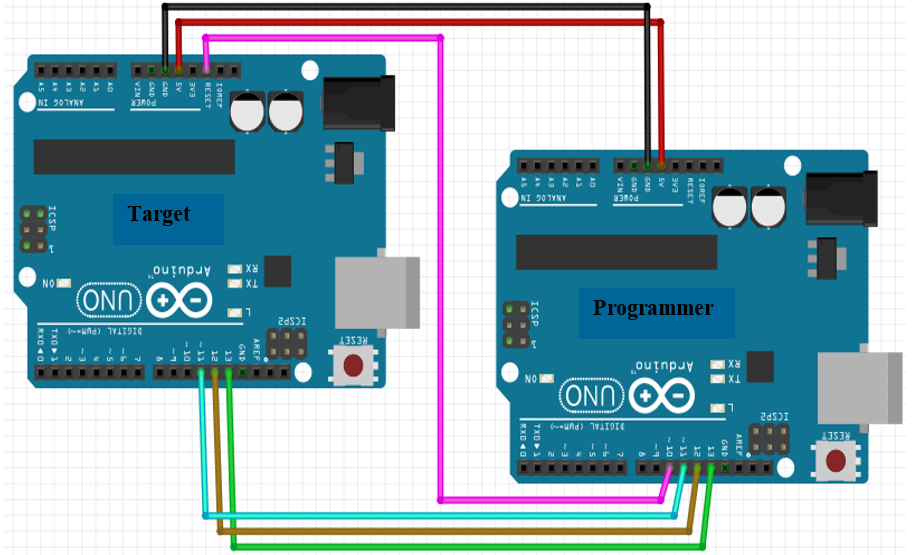
\includegraphics[scale=0.8]{EXP_27_Images/fig1.png}
\end{center}
\vspace{-10mm}
\begin{center} {Figure 1.Postman tool download}\end{center}
    
\item  After completion of the download, install it and make a free account.  After completion, a page similar to the given below will appear.    

\vspace{-3mm}
\begin{center} 
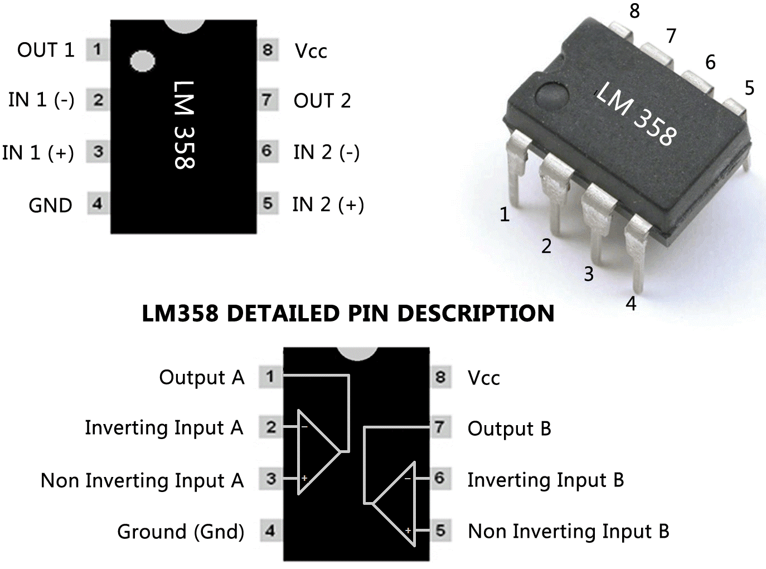
\includegraphics[scale=0.75]{EXP_27_Images/fig2.png}
\end{center}
\vspace{-5mm}
\begin{center} {Figure 2.Postman Workspaces page}\end{center}    
    
\end{enumerate}

\noindent \textbf{B)	Installation of Anaconda for Python (Jupyter IDE)}
\vspace{-5mm}
\begin{enumerate}
    \item Go to the link: https://www.anaconda.com. Inside the \textbf{Products} $ \rightarrow $ \ choose the \textbf{Individual Edition} and click on $ \rightarrow $ \ \textbf{Download}. While installing, choose $ \rightarrow $ \ \textbf{All users} option, and in \textbf{Advanced Options}, tick both the square boxes. At the end \textbf{uncheck} the \textbf{Anaconda Individual Edition Tutorial} and \textbf{Learn More about Anaconda} option boxes.
    \item After completing the installation, go to the \textbf{start menu} and search \textbf{Anaconda Navigator}. Click on it, a page similar to the given below will appear.

    \vspace{-5mm}
\begin{center} 
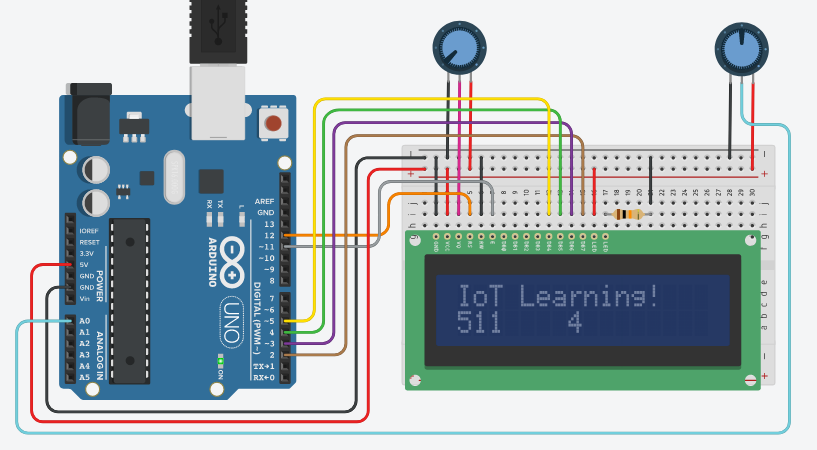
\includegraphics[scale=0.45]{EXP_27_Images/fig3.png}
\end{center}
\vspace{-7mm}
\begin{center} {Figure 3.Anaconda Navigator page}\end{center}  
    
\end{enumerate}




\noindent \textbf{C)	OM2M Server Setup}
\vspace{-3mm}
\begin{enumerate}
    \item Go to the link: http://wiki.eclipse.org/OM2M/Download. Click on the OM2M 1.4.1 Package to download the latest release as shown in fig.5 below.
    
\item After Successful download, extract the zip file "eclipse-om2m-v1-4-1.zip". There are two folders named \textbf{"in-cse"} and \textbf{"mn-cse"}.

\item Go to the \textbf{"in-cse"} folder $ \rightarrow $ \ and inside the \textbf{"configuration"} folder $ \rightarrow $ \ open \textbf{"config.ini"} file with notepad and in line 5 change the \textbf{port} to \textbf{5089}.

\item Now go to Command prompt (in Windows search for \textbf{"cmd"} in start, and open) or Terminal (Open a Linux Terminal Using \textbf{Ctrl + Alt + T }or search \textbf{Terminal} in Spotlight search in Mac OS). Once cmd/terminal opens \textbf{enter the command} $ \rightarrow $ \ \textbf{java-version}. Make sure you are in the right java-version since OM2M will only be compatible with \textbf{jdk 1.8.0\_X versions}. In case if you need to install jdk,  please refer to the below URLs based on the OS: \\[4pt]

Windows: https://codenotfound.com/java-download-install-jdk-8-windows.html \\[4pt]
Linux: https://docs.datastax.com/en/jdk-install/doc/jdk-install/installOpenJdkDeb.html \\[4pt]
Mac: https://stackoverflow.com/questions/24342886/how-to-install-java-8-on-mac

\begin{center} 
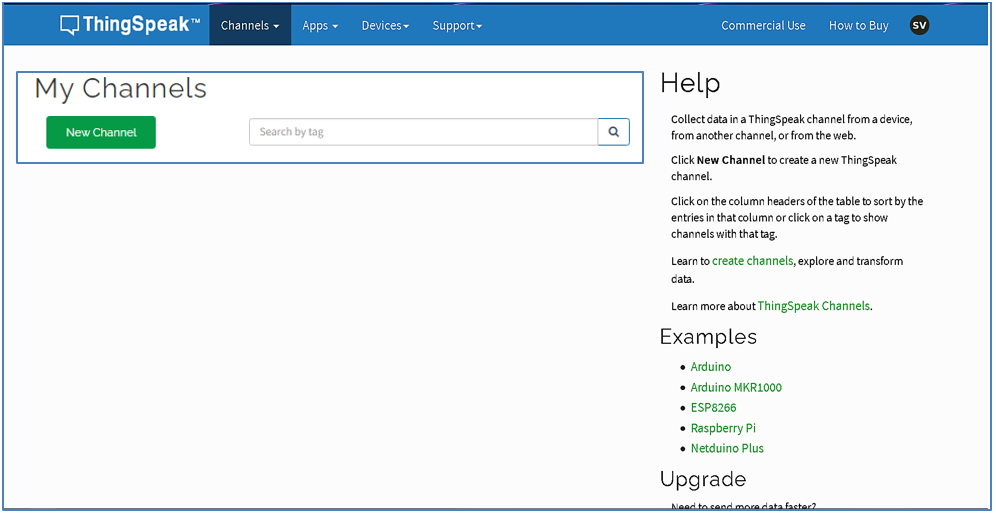
\includegraphics[scale=0.6]{EXP_27_Images/fig4.png}
\end{center}
\vspace{-9mm}
\begin{center} {Figure 4.OM2M Download page}\end{center}  

\item  Now open cmd/terminal and change the path using "cd" command to the \textbf{in-cse} folder of the previously downloaded OM2M 1.4.1 package (Make sure to provide the folder and its content with appropriate read and write permissions).

\begin{center} 
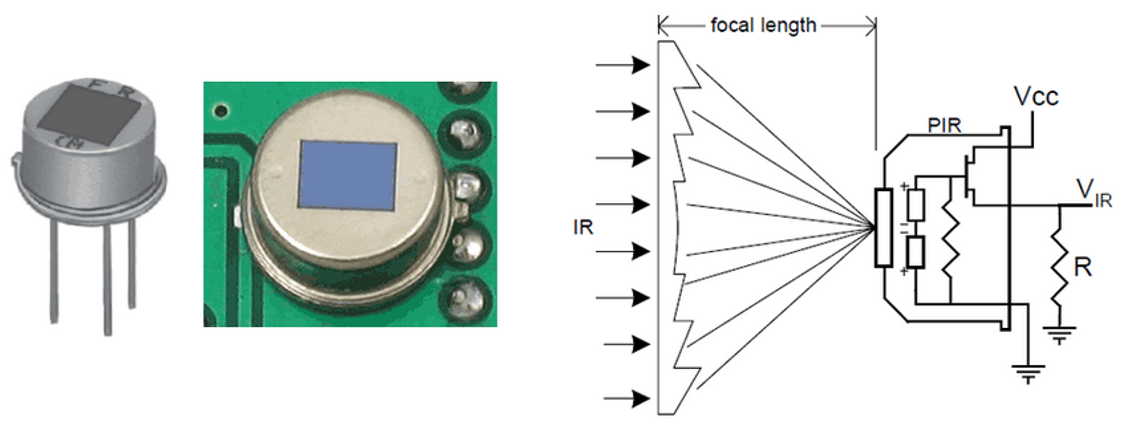
\includegraphics[scale=0.75]{EXP_27_Images/fig5.png}
\end{center}
\vspace{-9mm}
\begin{center} {Figure 5.Opening the \textbf{in-cse} folder}\end{center}  

\item  Now in cmd/terminal enter start.bat/start.sh to launch the OM2M in-cse interface. (Double click generally works as well inside the contents of in-cse folder, fig.6). Wait for the java command to get executed.

\begin{center} 
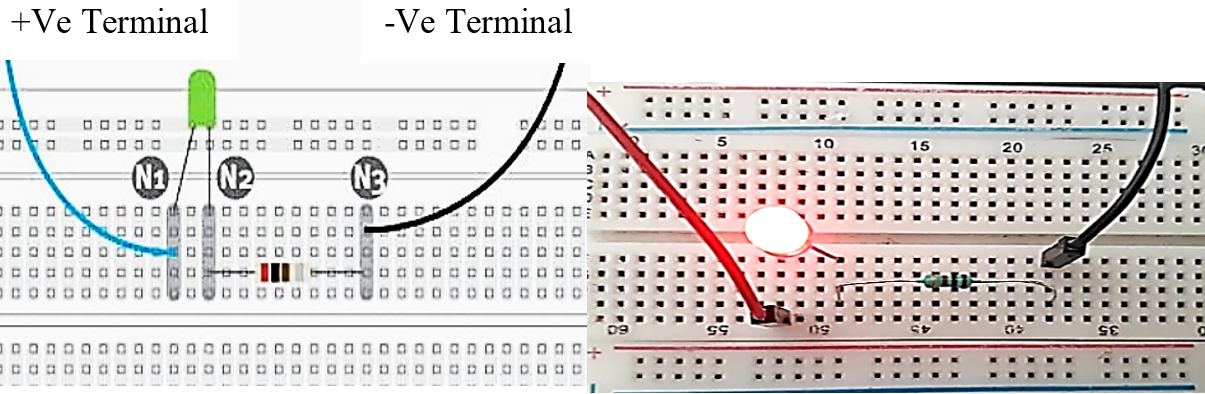
\includegraphics[scale=0.7]{EXP_27_Images/fig6.png}
\end{center}
\vspace{-9mm}
\begin{center} {Figure 6. Folder contents of in-cse folder}\end{center}  

\begin{center} 
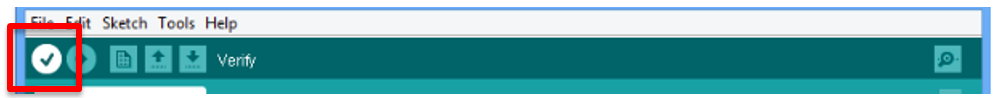
\includegraphics[scale=0.6]{EXP_27_Images/fig7.png}
\end{center}
\vspace{-9mm}
\begin{center} {Figure 7. Successful OM2M initialization}\end{center}  

\item Once the OM2M launches successfully as in fig.7, go to the OM2M login page using the link below, a page as given in fig.8 will appear. Link:  http://127.0.0.1:5089/webpage 

\begin{center} 
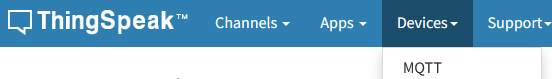
\includegraphics[scale=0.8]{EXP_27_Images/fig8.png}
\end{center}
\vspace{-9mm}
\begin{center} {Figure 8. OM2M Login page}\end{center}  

\item Enter the default \textbf {username} and \textbf {password} as \textbf{admin, admin}, and press login. We can see a default resource tree of OM2M as given in fig. 9 below.

\begin{center} 
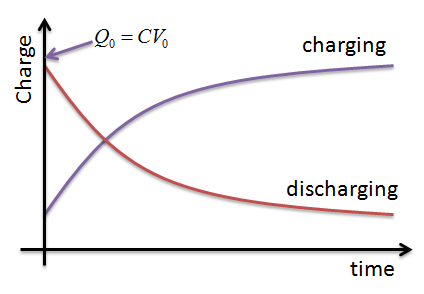
\includegraphics[scale=0.8]{EXP_27_Images/fig9.png}
\end{center}
\vspace{-7mm}
\begin{center} {Figure 9. Default Resource Tree of OM2M}\end{center} 
\end{enumerate}

\vspace{3cm}
\noindent \textbf{D)	Using Postman to create custom resources in postman}
\vspace{-3mm}
\begin{enumerate}
\item  Go to the Postman $ \rightarrow $ \ Workspaces $ \rightarrow $ \ Import $ \rightarrow $ \  Upload Files $ \rightarrow $ \ select the JSON files named as 'OM2M REST APIs.postman\_collection.json' and click on $ \rightarrow $ \ Import. We can see the request collections below the OM2M Rest APIs as shown in fig. 10 below.
    
    \begin{center} 
    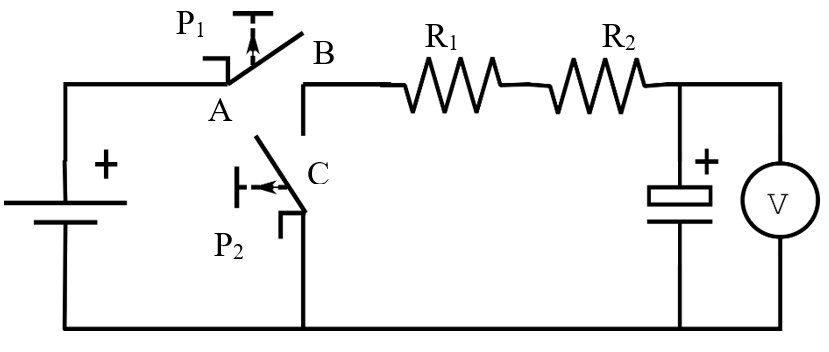
\includegraphics[scale=0.8]{EXP_27_Images/fig10.png}
    \end{center}
    \vspace{-7mm}
    \begin{center} {Figure 10.Collection of Requests after importing}\end{center} 
    
\item  Before using the collection make sure the OM2M server is running and available at http://127.0.0.1:5089/webpage.The request can be sent by pressing the "Send" button in postman, after selecting any particular request. Now we will send each request one by one to make the resource tree and store data. We can notice the changes in the OM2M server after each request by clicking on Tree nodes, and also notice the headers, body, and responses after each request in Postman. Following are the requests to be sent in steps, same as in fig.10.

    \begin{enumerate}
    \setlength\itemsep{-0.3em}
        \item Creating an Application Entity: Select $ \rightarrow $ \textcolor{orange}{Post} \textbf{Create Application Entity} $ \rightarrow $ Send
    \item Creating a container for device called Node-1: Select $ \rightarrow $ \textcolor{orange}{Post} \textbf{Create Node-1 container} $ \rightarrow $ Send
    \item Creating a Descriptor container: Select $ \rightarrow $ \textcolor{orange}{Post} \textbf{create descriptor cnt }$ \rightarrow $ Send
    \item Creating a Data container: Select $ \rightarrow $ \textcolor{orange}{Post} \textbf{Create Data container} $ \rightarrow $ Send
    \item Creating descriptor content instance: Select $ \rightarrow $ \textcolor{orange}{Post} \textbf{create descriptor cin }$ \rightarrow $ Send
    \item Creating data content instance 1 \& 2 : Select $ \rightarrow $ \textcolor{orange}{Post} \textbf{Create Content instance-1/2} $ \rightarrow $ Send
    \item Retrieving the latest content instance:  Select $ \rightarrow $ \textcolor{green}{GET} \textbf{latest Content instance} $ \rightarrow $ Send
    \item Retrieving the oldest content instance: Select $ \rightarrow $ \textcolor{green}{GET} \textbf{oldest Content instance} $ \rightarrow $ Send
    \item Retrieving all content instances: Select $ \rightarrow $ \textcolor{green}{GET} \textbf{all data of a container} $ \rightarrow $ Send
    \item pdating number of attributes inside data container: Select $ \rightarrow $ \textcolor{green}{PUT} \textbf{update cnt attrs} $ \rightarrow $ Send
    \item Deleting the resource:  Select $ \rightarrow $\textcolor{red}{DEL} \textbf {delete resource} $ \rightarrow $ Send
    \end{enumerate}
    
\end{enumerate}

\noindent \textbf{E) Interfacing IoT devices \& publishing data  to OM2M}

\noindent Connect the ESP32 to PC/Laptop and upload the script \textbf{'OneM2M.ino'}. For sake of simplicity, we are publishing random data from ESP32 but any sensor can be integrated and corresponding data can be published through ESP32 to the server of OM2M. We can see the data being published on the OM2M page.

\noindent \textbf{F) Data-Ware-Housing}

\noindent In this step, we are going to create an SQ-Lite3 database server through Python script. The script will create a folder named \textbf{'Database'} in the same directory where the Python script is located and inside that folder, a database is created. Follow the steps as given below.
\begin{enumerate}
    \item Open the \textbf{Jupyter Notebook} from \textbf{Anaconda Navigator}. In the \textbf{Home} page of Jupyter click on $ \rightarrow $ \textbf{Upload} and upload the file named \textbf{'Server4OM2M.ipynb'}. Open the file after uploading and click on \textbf{$ \rightarrow $ Kernel $ \rightarrow $ Restart \& Run All}.

\item The above steps only create a database server, now we have to connect it with OneM2M. Once the server is initialized and it is running, open the postman collection and select $ \rightarrow $ \textcolor{orange}{Post} \textbf{create subs} $ \rightarrow $ Send. Now, the data starts storing in the database once the subscription is established. We can retrieve data from the warehouse by selecting $ \rightarrow $ \textcolor{green}{GET} \textbf{Retrieve Data} $ \rightarrow $ Send, in the postman collection.
\end{enumerate}

\noindent \textbf{G) Visualizing the Stored Data in the Database}

\noindent In this step, we will connect the database with Jupyter notebook and create a simple dashboard to visualize the live data that is being pushed into the database. Firstly, make sure the device is constantly posting data to OM2M Server and the data is being stored in the Data Warehouse. Upload, open the Jupyter Notebook Script named \textbf{'Visualize\_SDB.ipynb'}, and run all the cells
like the data warehouse script. Once the script runs successfully, dynamic graphs are generated based on the number of parameters in the om2m descriptor.\\[6pt]

\noindent \textbf{\large REFERENCES:}
\vspace{-3mm}
\begin{enumerate}
\setlength\itemsep{-0.3em}
\item  \href {https://wiki.eclipse.org/OM2M/one/REST_API#Create_a_.22MY_SENSOR.22_application}{OM2M/one/REST API}
\end{enumerate}

\end{justify}
\end{document}